\documentclass[12pt]{article}

% packages
\usepackage[margin=1in]{geometry}
\usepackage[labelfont=it]{caption}
\usepackage{subcaption}
\usepackage{framed}
\usepackage[table]{xcolor}
\usepackage{colortbl, multirow, placeins}
\usepackage{amsmath,amsthm,amssymb,wasysym}
\usepackage{mathrsfs, mathtools}
\usepackage{tikz,pgf,pgfplots,pgffor}
\pgfplotsset{compat=1.16}
\usetikzlibrary{arrows, angles, quotes, decorations.pathreplacing, math, patterns, calc}
\usepackage{graphicx}

% custom commands
\newcommand{\N}{\mathbb{N}}
\newcommand{\Z}{\mathbb{Z}}
\newcommand{\I}{\mathbb{I}}
\newcommand{\R}{\mathbb{R}}
\newcommand{\Q}{\mathbb{Q}}
\newcommand{\p}{^{\prime}}
\DeclarePairedDelimiter{\ceil}{\lceil}{\rceil}
\DeclarePairedDelimiter{\floor}{\lfloor}{\rfloor}

 
\begin{document}
 
\title{Game of Nim\\
    \large MATH CS 101A Problem Solving I}
\author{Harry Coleman}
\date{December 3, 2019}

\maketitle

\begin{framed}\noindent
    \textbf{Problem:} There are several piles of beans on the table. Two persons take turn. A move consists of selecting a heap and removing any number of beans from it, but at least one. The player who takes the last bean wins. Which of the two players has a winning strategy? Which one is it? (Hint: use binary representation of the number of beans in each heap.)
\end{framed}

\section{Nim States}
In this document, we will consider games of Nim with a finite, nonnegative, integer number of piles of beans, each pile with a finite, nonnegative, integer number of beans. We will not explore infinite, negative, or non-integral quantities of piles or the beans therein. We will consider a \emph{state} in the game of Nim to be an arrangement of some number of beans into some piles. 
\begin{figure}[ht]
    \centering
    \begin{subfigure}[b]{.47\textwidth}
        \centering
        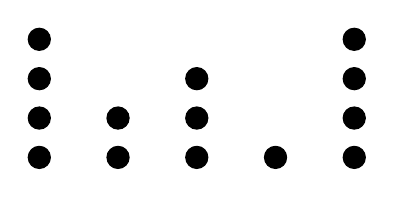
\begin{tikzpicture}
            \foreach \x / \up in {0/4,1/2,2/3,3/1,4/4}
                \foreach \y in {1,...,\up}
                     \draw[fill=black] (\x,\y/2) circle (4pt);
        \end{tikzpicture}
        \caption{Some piles of beans.}
        \label{fig:bean-example-1}
    \end{subfigure}
    \begin{subfigure}[b]{.47\textwidth}
        \centering
        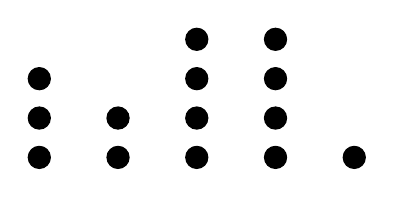
\begin{tikzpicture}
            \foreach \x / \up in {0/3,1/2,2/4,3/4,4/1}
                \foreach \y in {1,...,\up}
                     \draw[fill=black] (\x,\y/2) circle (4pt);
        \end{tikzpicture}
        \caption{Some more piles of beans.}
        \label{fig:bean-example-2}
    \end{subfigure}
    \caption{beep boop beans}
    \label{fig:bean-examples}
\end{figure}

In the case of Figure \ref{fig:bean-example-1}, we have a pile of four beans, followed by a pile of two beans, then a pile of three beans, then a pile of one bean, and finally a pile of four beans. Because it's possible for multiple piles to have the same number of beans, we would not want to use sets to represent these piles of beans. Instead, we will use ordered tuples. so we would represent the state in Figure \ref{fig:bean-example} by $(4,2,3,1,4)$. Consider, now, the state shown in Figure \ref{fig:bean-example-2}.



\begin{figure}[ht]
    \centering
    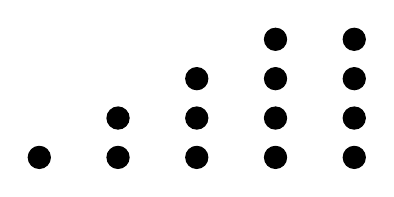
\begin{tikzpicture}
        \foreach \x / \up in {0/1,1/2,2/3,3/4,4/4}
            \foreach \y in {1,...,\up}
                 \draw[fill=black] (\x,\y/2) circle (4pt);
    \end{tikzpicture}
    \caption{The bean piles of Figure \ref{fig:bean-example}, but reordered.}
    \label{fig:bean-example-sort}
\end{figure}

Because the rules of Nim make no mention of the arrangement of piles, Figures \ref{fig:bean-example} and \ref{fig:bean-example-2} would simply be different representations of the same state with respect to Nim. So each state has a number of possible permutations on the order of the piles. We will assume, without loss of generality, that when we refer to the order of the piles, they are ordered by "$\leq$" on the number of beans in each pile. So the state represented by Figures \ref{fig:bean-example} and \ref{fig:bean-example-2} will instead be represented by Figure 



For the rest of the document, we will consider there to be an arbitrary $n\in\N$ number of piles in all our states. Since we can have piles with zero beans, this will also consider all states with less than $n$ non-zero piles. So we will define our set of indices,
\begin{equation}
    I = \{i\in\N: i\leq n\} = \{1, 2, 3, \dots, n\}.
\end{equation}

We represent a state, $S$, with the indexed family
\begin{equation}
    (s_i)_{i\in I},
\end{equation}
where $s_i$ gives the number of beans in the $i$th pile of $S$. 


\[K(S) = \max\{k_1,\dots,k_n\},\]
which is the number of beans in the largest pile(s) in $S$. So $K(S)\in S$ and for all $k_i\in S$, $k_i\leq K(S)$.

If a player's turn starts with the game in the state $S$, that player takes an \emph{action} that involves decreasing one of the piles, say $k_j$, by a whole number no less than 1 and no more than $k_j$. This action moves the game from the state $S$ to 
\begin{center}
    $S' = S$ with $k_j$ replaced with $k_j'$.
\end{center}
where $k_j'$ is some integer such that $0\leq k_j' < k_j$. It then becomes the opposite player's turn, who must take an action on $S'$. We consider the player who takes an action on the current game state $S$ that produces $S'$ such that all elements in $S'$ are zero (i.e. takes the last bean, leaving all empty piles). Because of this, we will consider the state of all zeros, $(0,\dots,0)$, to be the \emph{ultimate loss state}, since a player who starts their turn in this state has lost the game.

In general, we will consider a \emph{loss state} to be one which, assuming perfect strategy by both players, will result in a loss for the player which starts a turn in that state. In other words, a loss state is one in which every possible action will result in a \emph{win state} for the opposite player. In general, a win state is one in which there exists an action which will result in a loss state for the opposite player.

These definitions could be applied to all of our states, recursively, with the ultimate loss state explicitly defined. However, this process is fairly computationally complex for large $n$ and $k$'s. We will instead show that we can determine whether a state is a win state or a loss state using a property independent of other states.

\section{Lattice Representation of States}
This section is not crucial to the proof, but presents an interesting way of conceptualizing the game of Nim. Since all of our states are tuples of natural numbers, we can imagine all possible states as all the integral lattice points in $n$-dimensional euclidean space. For simplicity, we will look at the case of $n=2$, so all of our states are of the form $(k_1,k_2)$ where both $k_1,k_2 \in \N\cup\{0\}$.
\begin{center}
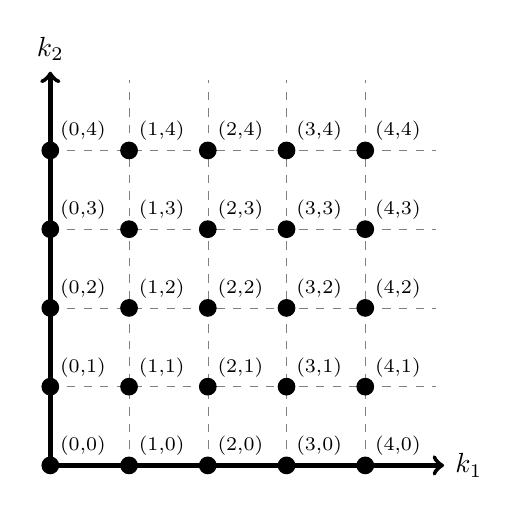
\begin{tikzpicture}
    \draw[help lines, color=gray, dashed] (0,0) grid (4.9,4.9);
    \draw[->,ultra thick] (0,0)--(5,0) node[right]{$k_1$};
    \draw[->,ultra thick] (0,0)--(0,5) node[above]{$k_2$};
    
    \foreach \x in {0,1,2,3,4} {
        \foreach \y in {0,1,2,3,4} {
            \draw[fill=black] (\x,\y) circle (3pt) node[anchor=south west] {\scriptsize (\x,\y)};
        }
    }
\end{tikzpicture}
\end{center}

We can see that every state where $k_1$ and $k_2$ are less than or equal to 4 occur in this lattice. Consider now, the state $A = (3,2)$, and the possible $A'$ that are obtainable from a single action on $A$. We find that $A'\in\{(2,2),(1,2),(0,2),(3,1),(3,0)\}$. On the graph,
\begin{center}
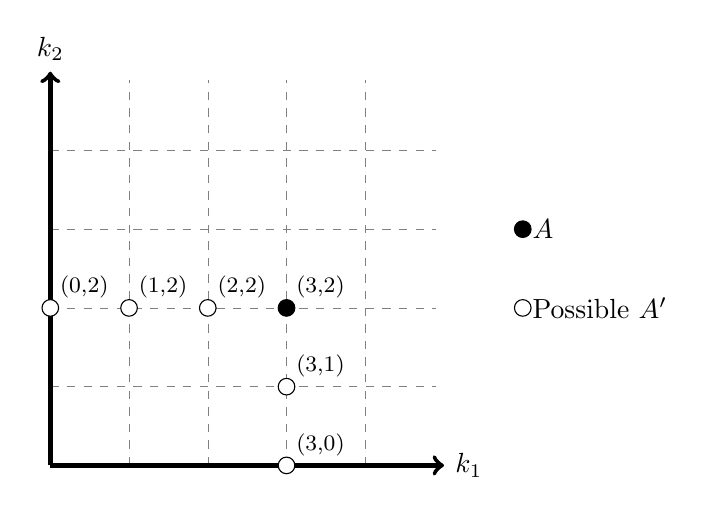
\begin{tikzpicture}
    \draw[help lines, color=gray, dashed] (0,0) grid (4.9,4.9);
    \draw[->,ultra thick] (0,0)--(5,0) node[right]{$k_1$};
    \draw[->,ultra thick] (0,0)--(0,5) node[above]{$k_2$};
    
    \draw[fill=black] (3,2) circle (3pt) node[anchor=south west] {\footnotesize (3,2)};
    
    \draw[fill=white] (0,2) circle (3pt) node[anchor=south west] {\footnotesize (0,2)};
    \draw[fill=white] (1,2) circle (3pt) node[anchor=south west] {\footnotesize (1,2)};
    \draw[fill=white] (2,2) circle (3pt) node[anchor=south west] {\footnotesize (2,2)};
    \draw[fill=white] (3,1) circle (3pt) node[anchor=south west] {\footnotesize (3,1)};
    \draw[fill=white] (3,0) circle (3pt) node[anchor=south west] {\footnotesize (3,0)};
    
    \draw[fill=black] (6,3) circle (3pt) node[anchor=west]{$A$};
    \draw[fill=white] (6,2) circle (3pt) node[anchor=west]{Possible $A'$};
\end{tikzpicture}
\end{center}
it becomes clear that an action on a state, in the graph, is a movement towards the origin, parallel to one of the axes. This is because an action on a state involves decreasing exactly one element of the state's tuple, leaving all other elements unchanged. So taking each element to be one of the axes in the graph means that we always move parallel to the axis whose element we are decreasing.

It can also be seen that our definition of states as tuples results in states with multiple representations as tuples. For instance, $(1,3)$ and $(3,1)$ are different tuples, but would be equivalent games of Nim, since the order of piles in irrelevant in Nim. In fact, in the case of $n=2$, any two states which have reflexive symmetry across the line $k_2=k_1$ are equivalent in Nim.

\section{Computer Program}
Again, this section is not crucial for the proof, but will provide context and motivation for the proof. A computer program was used to generate win and loss states based on their lattice representations and the recursive definition of win and loss states. Recall the definition,

\begin{framed}
    \begin{tabular}{r l l}
        \multicolumn{3}{l}{For a given state $S$,} \\
        (i) & $S$ is a loss state & if it is the ultimate loss state (i.e. all zeros $(0,\dots,0)$). \\ 
        (ii) & $S$ is a loss state & if \textbf{for every action} from $S$ to $S'$, $S'$  a win state. \\
        (iii) & $S$ is a win state & \multirow{2}{\textwidth}{if \textbf{there exists an action} from $S$ to $S'$, such that\\$S'$ is a loss state.} \\
    \end{tabular}
    \\\\
\end{framed}

Consider, again, the case of $n=2$. By (i), we see that that the origin is a loss state, since it is the ultimate loss state. On the graph, this looks like
\begin{center}
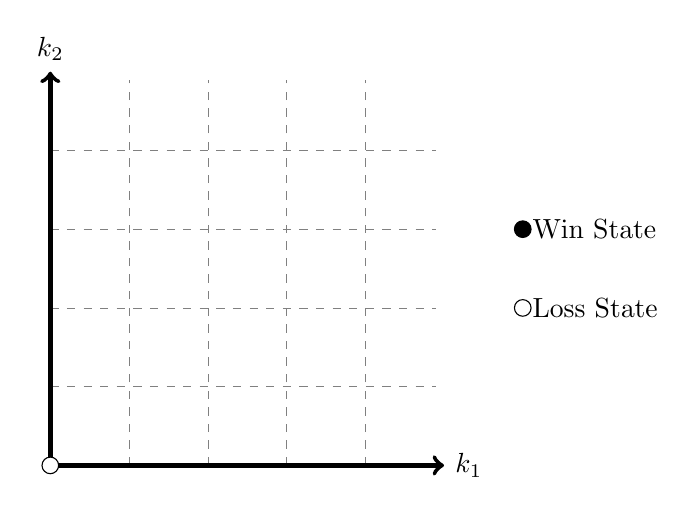
\begin{tikzpicture}
    \draw[help lines, color=gray, dashed] (0,0) grid (4.9,4.9);
    \draw[->,ultra thick] (0,0)--(5,0) node[right]{$k_1$};
    \draw[->,ultra thick] (0,0)--(0,5) node[above]{$k_2$};
    
    \draw[fill=white] (0,0) circle (3pt);
    
    \draw[fill=black] (6,3) circle (3pt) node[anchor=west]{Win State};
    \draw[fill=white] (6,2) circle (3pt) node[anchor=west]{Loss State};
\end{tikzpicture}
\end{center}

Then, by (iii), we find that all of the points along the axes are win states, since from any of these points, there exists an action (moving along the axis it is on) which obtains a loss state (the origin). 

\begin{center}
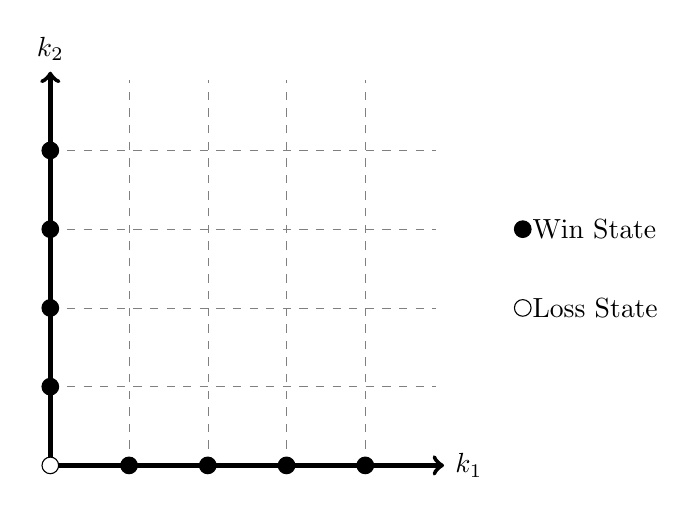
\begin{tikzpicture}
    \draw[help lines, color=gray, dashed] (0,0) grid (4.9,4.9);
    \draw[->,ultra thick] (0,0)--(5,0) node[right]{$k_1$};
    \draw[->,ultra thick] (0,0)--(0,5) node[above]{$k_2$};
    
    \draw[fill=black] (6,3) circle (3pt) node[anchor=west]{Win State};
    \draw[fill=white] (6,2) circle (3pt) node[anchor=west]{Loss State};
    
    \draw[fill=white] (0,0) circle (3pt);
    
    \foreach \i in {1,2,3,4} {
        \draw[fill=black] (\i,0) circle (3pt);
        \draw[fill=black] (0,\i) circle (3pt);
    }
\end{tikzpicture}
\end{center}

We then consider the state $(1,1)$, which can move to either $(1,0)$ or $(0,1)$, both of which are win states. So by (ii), we find $(1,1)$ to be a loss state. Continuing this process of assigning win or loss to states once they satisfy one of the properties, we find the graph to be filled out in the following way.

\begin{center}
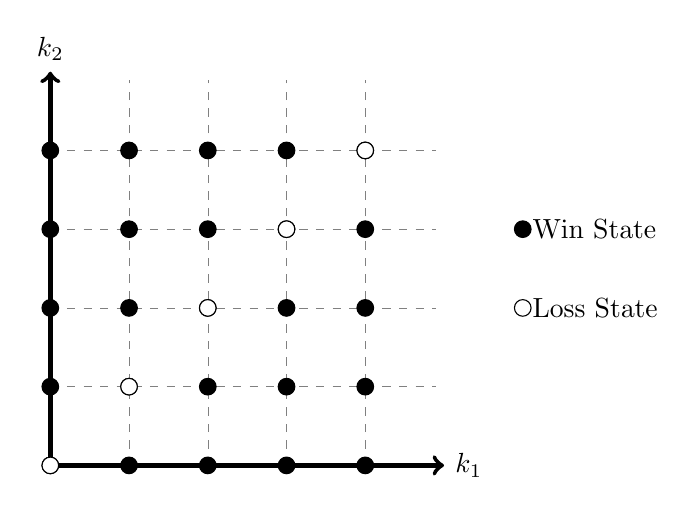
\begin{tikzpicture}
    \draw[help lines, color=gray, dashed] (0,0) grid (4.9,4.9);
    \draw[->,ultra thick] (0,0)--(5,0) node[right]{$k_1$};
    \draw[->,ultra thick] (0,0)--(0,5) node[above]{$k_2$};
    
    \draw[fill=black] (6,3) circle (3pt) node[anchor=west]{Win State};
    \draw[fill=white] (6,2) circle (3pt) node[anchor=west]{Loss State};
    
    
    \foreach \x in {0,1,2,3,4} {
        \foreach \y in {0,1,2,3,4} {
            \draw[fill=black] (\x,\y) circle (3pt);
        }
        \draw[fill=white] (\x,\x) circle (3pt);
    }
\end{tikzpicture}
\end{center}

The program would fill out a graph based on a fixed $n$ and $k_{\text{max}}$ (all $k_i \leq k_{\text{max}}$). Such a graph would have $(k_{\text{max}})^n$ possible states to fill out. However, as previously mentioned, many Nim games have multiple representations as tuples, so we are able to cut down the size of this graph by defining equivalence classes for such states. Two states are considered equivalent if their \emph{sorted} tuple representations are the same. Given a state
\[S = (k_1, k_2, k_3, \dots, k_n)\]
we define the sorted tuple representation to be the tuple
\[O(S) = (l_1, l_2, l_3, \dots, l_n)\]
such that $l_1 \leq l_2 \leq l_3 \leq \cdots \leq l_n$ and there exists a bijection, $f$, between the indices of $S$, $\{i\in\N: i\leq n\}$, and the indices of $O(S)$, $\{j\in\N: j\leq n\}$, where $f(i) = j$ tells us that $k_i=l_j$. Intuitively, $O(S)$ is a reordering of $S$ from least to greatest. For example, if we have the state $A = (5,4,2,3,2,4) \text{, then } O(A) = (2,2,3,4,4,5)$. We then consider two states to be equivalent if and only if their sorted tuple representations are equal. That is, for any two states $A$ and $B$,
\[A \equiv B \iff O(A) = O(B)\]

And we can then find for any state $S$, we find the equivalence class
\[[S] = \{A: O(S) = O(A)\}\]
and take the canonical form of $[S]$ to be $O(S)$. Consider the state $A = (2,3,1)$, we find that
\[[A] = \{(1,2,3), (3,1,2), (2,3,1), (3,2,1), (1,3,2), (2,1,3)\}\]
with the canonical form $(1,2,3)$. With this, we simplify the number of cases the program needs to check from \[(k_{\text{max}})^n \qquad \text{to} \qquad \binom{n+k_{\text{max}}}{k_{\text{max}}} = \frac{(n+k_{\text{max}})!}{n!k_{\text{max}}!}\]
\begin{center}
    (The proof is left as an exercise to the reader.)
\end{center}

We let the program evaluate win and loss states up to $n=10$ and $k_{max}=10$. Using the naive representation of states, this would be $10^{10}$ states, but simplifying to sorted tuple representations allows the evaluation of less than $2\cdot 10^5$ equivalent states. We then looked at the binary representations of a number of loss and win states, noting the differences. These observations serve as the motivation for the definition presented in the next section.

\section{Parity of States}
We will now define, for each of our states, a property which we will call its \emph{parity}. To find the parity of a state
\[S = (k_1, k_2, k_3, \dots, k_n)\]
we construct the following table.
\begin{center}
    \rowcolors{1}{white}{gray!10}
    \begin{tabular}{l|cccc}
         & $k_1$ & $k_2$ & $\dots$ & $k_n$ \\
         \hline
        \cellcolor{white} $2^0$ & $a_{10}$ & $a_{20}$ & $\dots$ & $a_{n0}$ \\
        \cellcolor{white} $2^1$ & $a_{11}$ & $a_{21}$ & $\dots$ & $a_{n1}$ \\
        \cellcolor{white} $2^2$ & $a_{12}$ & $a_{22}$ & $\dots$ & $a_{n2}$ \\
        $\vdots$ & $\vdots$ & $\vdots$ & $\dots$ & $\vdots$
    \end{tabular}
\end{center}

In the table, each $a_{ij}$ is the $j$th digit from the right in the binary representation of $k_i$. Equivalently, we can define
\[a_{ij} = \floor*{\frac{k_i}{2^j}} \bmod 2\]
where $a_{ij} = 1$ if $2^j$ is part of the binary representation for $k_i$, and $a_{ij} = 0$, otherwise. 

\newpage
For example, we could construct a table for the state
\[A = (3,4,5,6,7)\]
\begin{center}
    \rowcolors{1}{white}{gray!10}
    \begin{tabular}{c|ccccc}
         & 3 & 4 & 5 & 6 & 7 \\
         \hline
        \cellcolor{white} $2^0$ & 1 & 0 & 1 & 0 & 1 \\
        \cellcolor{white} $2^1$ & 1 & 0 & 0 & 1 & 1 \\
        \cellcolor{white} $2^2$ & 0 & 1 & 1 & 1 & 1
    \end{tabular}
\end{center}

It can be seen that the binary representation of each number is it's column read bottom to top. We will now define $r_j$ to be the sum of all the entries in the row labelled $2^j$. The formula is given as
\[r_j = \sum_{i=1}^n a_{ij}\]

So in our example of $A$, we would have
\[r_0 = 3 \qquad r_1 = 3 \qquad r_2 = 4 \]

Finally, we define a predicate which gives us the parity of state $S$.
\[
    \text{Parity of } S = 
    \begin{cases}
        \text{even} & \text{if all $r_j$ in the table for $S$ are even.}\\
        \text{odd} & \text{otherwise (if at least one $r_j$ in the table for $S$ is odd).}
    \end{cases}
\]

Since in the table for $A$, we have at least one $r_j$ odd (both $r_0$ and $r_1$ are odd), $A$ is an odd state. If, instead, we considered the state
\[B = (3,4,5,6,11,15)\]
\begin{center}
    \rowcolors{1}{white}{gray!10}
    \begin{tabular}{c|cccccc|c}
         & 3 & 4 & 5 & 6 & 11 & 15 & $r_j$ \\
         \hline
        \cellcolor{white} $2^0$ & 1 & 0 & 1 & 0 & 1 & 1 & 4 \\
        \cellcolor{white} $2^1$ & 1 & 0 & 0 & 1 & 1 & 1 & 4 \\
        \cellcolor{white} $2^2$ & 0 & 1 & 1 & 1 & 0 & 1 & 4 \\
        \cellcolor{white} $2^3$ & 0 & 0 & 0 & 0 & 1 & 1 & 2
    \end{tabular}
\end{center}
we find that $B$ is an even state since all $r_0, r_1, r_2, r_3$ are even. Equivalently, we can say that all $r_j$ are even, and therefore $S$ is even, if and only if 
\[\sum_{j=0}^\infty(r_j \bmod 2) = 0\]

So if we define, for a given state $S = (k_1, k_2, k_3, \dots, k_n)$,
\[R(S) = \sum_{j=0}^\infty\left(\left(\sum_{i=1}^n \floor*{\frac{k_i}{2^j}}\right) \bmod 2\right)\]
then we say that $S$ is even if and only if $R(S) = 0$. More simply, we might consider the bitwise-exclusive-or operator($\oplus$) applied to all the elements of $S$. If we define
\[X(S) = k_1 \oplus k_2 \oplus k_3 \oplus \cdots \oplus k_n\]
then we can look at the equivalent form
\[X(S) = \sum_{j=0}^\infty 2^j \left(\left(\sum_{i=1}^n \floor*{\frac{k_i}{2^j}}\right) \bmod 2\right)\]

We notice that $R(S)$ and $X(S)$ differ only for nonzero values. So $S$ is even $\iff R(S)=0 \iff X(S)=0$. Either $R(S)$ or $X(S)$ can be used to determine the parity of a state. $X(S)$ may be a more typical operation, however, we will be using the tables associated with states in the derivation of $R(S)$ to help with the proof.

Next, we will consider how the relationship between the parity of $S$ and $S'$, where $S'$ is a state resulting from some action on $S$.

\section{Actions on Even States}
We will first consider an arbitrary even state, $S$. We consider some action on $S$, where we select some $k_i\in S$, and obtain $S'$ which is has all the same elements as $S$, except $k_i$ is replaced with $k_i'$ such that $0\leq k_i' < k_i$. Based on this, we want to say something about the parity of $S'$. Recall the table used to calculate $R(S)$,
\begin{center}
    \rowcolors{1}{white}{gray!10}
    \begin{tabular}{l|cccccc|c}
         & $k_1$ & $k_2$ & $\dots$  & $k_i$ & $\dots$& $k_n$ & \\
         \hline
        \cellcolor{white} $2^0$ & $a_{10}$ & $a_{20}$ & $\dots$ & $a_{i0}$ & $\dots$ & $a_{n0}$ & $r_0$ \\
        \cellcolor{white} $2^1$ & $a_{11}$ & $a_{21}$ & $\dots$ & $a_{i1}$ & $\dots$ & $a_{n1}$ & $r_1$ \\
        \cellcolor{white} $2^2$ & $a_{12}$ & $a_{22}$ & $\dots$ & $a_{i2}$ & $\dots$ & $a_{n2}$ & $r_2$ \\
        $\vdots$ & $\vdots$ & $\vdots$ & $\dots$ & $\vdots$ & $\dots$ & $\vdots$ & $\vdots$
    \end{tabular}
\end{center}

Likewise, the table for $S'$,
\begin{center}
    \rowcolors{1}{white}{gray!10}
    \begin{tabular}{l|cccccc|c}
         & $k_1$ & $k_2$ & $\dots$  & $k_i'$ & $\dots$& $k_n$ & \\
         \hline
        \cellcolor{white} $2^0$ & $a_{10}$ & $a_{20}$ & $\dots$ & $a_{i0}'$ & $\dots$ & $a_{n0}$ & $r_0'$ \\
        \cellcolor{white} $2^1$ & $a_{11}$ & $a_{21}$ & $\dots$ & $a_{i1}'$ & $\dots$ & $a_{n1}$ & $r_1'$ \\
        \cellcolor{white} $2^2$ & $a_{12}$ & $a_{22}$ & $\dots$ & $a_{i2}'$ & $\dots$ & $a_{n2}$ & $r_2'$ \\
        $\vdots$ & $\vdots$ & $\vdots$ & $\dots$ & $\vdots$ & $\dots$ & $\vdots$ & $\vdots$
    \end{tabular}
\end{center}

Since $k_i \ne k_i'$, then their binary representations are not the same, so there exists some $j$ such that $a_{ij} \ne a_{ij}'$. And because all $a$ values are 1 or 0, we know that
\begin{align*}
    a_{ij}=0 &\implies a_{ij}'= 1 \text{ so } r_j + 1 = r_j' \\
    a_{ij}=1 &\implies a_{ij}'= 0 \text{ so } r_j - 1 = r_j'
\end{align*}

Since $S$ is even, $r_j$ is even. So $r_j \pm 1 = r_j'$ is odd, making $S'$ is odd. So we can say that if $S$ is an even state, then any action on $S$ will produce an $S'$ that is an odd state.

\newpage
\section{Actions on Odd States}
We now consider an arbitrary odd state, $S$. 


\begin{table}[h!]
    \centering
    \rowcolors{1}{white}{gray!10}
    \begin{tabular}{l|cccccc|c}
         & $k_1$ & $k_2$ & $\dots$  & $k_i$ & $\dots$& $k_n$ & \\
         \hline
        \cellcolor{white} $2^0$ & $a_{10}$ & $a_{20}$ & $\dots$ & $a_{i0}$ & $\dots$ & $a_{n0}$ & $r_0$ \\
        \cellcolor{white} $2^1$ & $a_{11}$ & $a_{21}$ & $\dots$ & $a_{i1}$ & $\dots$ & $a_{n1}$ & $r_1$ \\
        \cellcolor{white} $2^2$ & $a_{12}$ & $a_{22}$ & $\dots$ & $a_{i2}$ & $\dots$ & $a_{n2}$ & $r_2$ \\
        $\vdots$ & $\vdots$ & $\vdots$ & $\dots$ & $\vdots$ & $\dots$ & $\vdots$ & $\vdots$ \\
    \end{tabular}
    \caption{Bean Analysis Values for $S$}
    \label{table:peen}
\end{table}

We'll define $J_{odd} = \{j: r_j \text{ is odd}\}$. We know that this set is nonempty, since $S$ is an odd state. 


\end{document}